%%% This LaTeX source document can be used as the basis for your technical
%%% report. Intentionally stripped and simplified
%%% and commands should be adjusted for your particular paper - title, 
%%% author, citations, equations, etc.
% % Citations/references are in report.bib 

\documentclass[conference]{acmsiggraph}

\usepackage{graphicx}
\graphicspath{{./images/}}
\newcommand{\figuremacroW}[4]{
	\begin{figure}[h] %[htbp]
		\centering
		\includegraphics[width=#4\columnwidth]{#1}
		\caption[#2]{\textbf{#2} - #3}
		\label{fig:#1}
	\end{figure}
}

\newcommand{\figuremacroF}[4]{
	\begin{figure*}[h] % [htbp]
		\centering
		\includegraphics[width=#4\textwidth]{#1}
		\caption[#2]{\textbf{#2} - #3}
		\label{fig:#1}
	\end{figure*}
}


\usepackage{lipsum}

\usepackage{xcolor}
\definecolor{lbcolor}{rgb}{0.98,0.98,0.98}
\usepackage{listings}

\lstset{
	escapeinside={/*@}{@*/},
	language=C,
	basicstyle=\fontsize{8.5}{12}\selectfont,
	numbers=left,
	numbersep=2pt,    
	xleftmargin=2pt,
	%numberstyle=\tiny,
	frame=tb,
	%frame=single,
	columns=fullflexible,
	showstringspaces=false,
	tabsize=4,
	keepspaces=true,
	showtabs=false,
	showspaces=false,
	%showstringspaces=true
	backgroundcolor=\color{lbcolor},
	morekeywords={inline,public,class,private,protected,struct},
	captionpos=t,
	lineskip=-0.4em,
	aboveskip=10pt,
	%belowskip=50pt,
	extendedchars=true,
	breaklines=true,
	prebreak = \raisebox{0ex}[0ex][0ex]{\ensuremath{\hookleftarrow}},
	keywordstyle=\color[rgb]{0,0,1},
	commentstyle=\color[rgb]{0.133,0.545,0.133},
	stringstyle=\color[rgb]{0.627,0.126,0.941},
}


\TOGonlineid{45678}
\TOGvolume{0}
\TOGnumber{0}
\TOGarticleDOI{1111111.2222222}
\TOGprojectURL{}
\TOGvideoURL{}
\TOGdataURL{}
\TOGcodeURL{}

\title{Computer Graphics Final Report}

\author{Sam Serrels\\\ 40082367@napier.ac.uk \\
Edinburgh Napier University\\
Computer Graphics (SET08116)}
\pdfauthor{Sam Serrels}

\keywords{OpenGL, GLSL, Graphics, SSBO, Reflections}

\begin{document}

\teaser{
   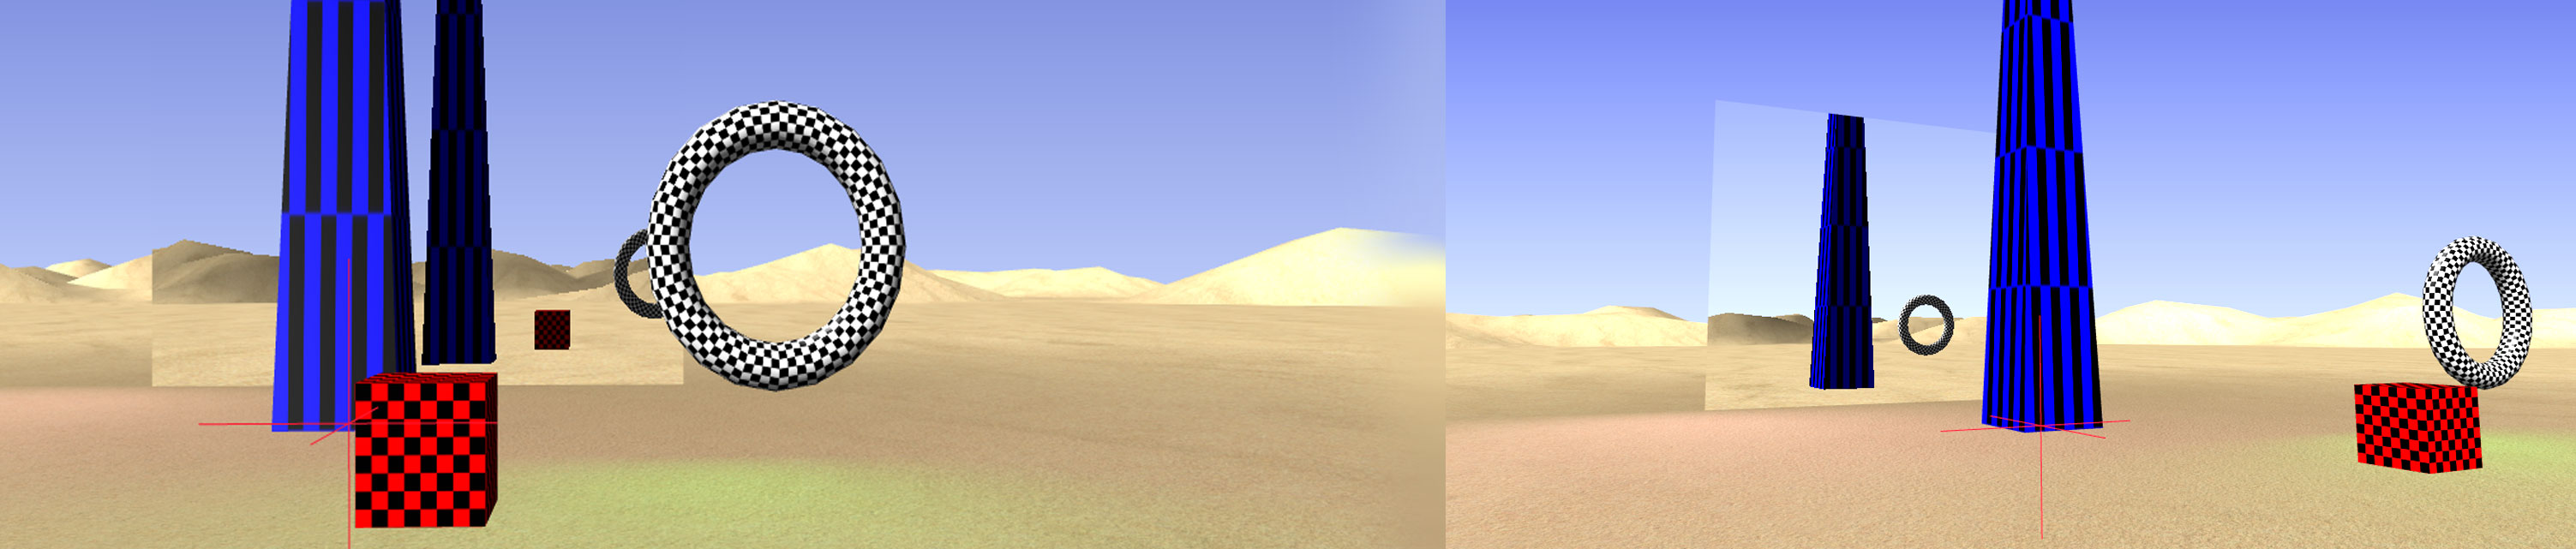
\includegraphics[height=1.5in]{images/sampleteaser}
   \caption{Project screenshot}   
 }		

\maketitle

\begin{abstract}
This project aims to develop a Real-time 3D graphics scene, with an emphasis on high aesthetic quality. The scene will use a pre-written OpenGL render framework to save development time for producing graphical effects. This project aims to also look into the cutting edge features available in the newest OpenGL standards and investigate the performance benefits of such features.
\end{abstract}

\keywordlist
%\copyrightspace

\section{Introduction}

\figuremacroW
{witness}
{Project Inspiration - The Witness}
{\protect\cite{Witness}}
{1.0}

\paragraph{Project Aims}
The setting for the project scene is a Desert. Although not a visually busy scene, a desert provides vibrant and harsh lighting, interesting landscape and plenty of opportunity to squeeze more visual fidelity out of a small amount of scene elements.
Using a multitude of texture effects, such as bump and parallax mapping, blend maps and level-of-detail, this project plans to bring life to even the most basic of objects, like sand on the ground.

\paragraph{Sky}
With the wide open vita of a desert plain, the sky takes center stage and is the most important visual cue to selling the realism of the scene. This project aims to have a fully dynamic and procedural sky system, without relying on static textures. This will allow for a time-of day system and full control of elements such as clouds and sun position.

\paragraph{Water}
The centrepiece of the scene will be a water feature of some kind, providing a contrast against the dry desert and a visually interesting element in it's own right. Reflections, waves using distortion maps, refraction, and particle effects will be used to provide realistic looking water. 

\section{Background / Related Work}
\figuremacroW
{specops}
{Spec Ops: The Line}
{\protect\cite{spec}}
{1.0}
Desert scenes are not uncommon to video games, the  simplicity of the landscape was a large bonus to performance limited software.
Older games (pre DirectX 9), could get away with a simple ground mesh, a single sand texture and an interesting skybox, and this would be considered a sufficiently detailed scene for the time. See Figure: \ref{fig:GuildWars}
\\
As the graphical power of computers increased, the challenges to make a realistic desert increased dramatically, the standard of games required more than just a barren wasteland. Buildings, foliage, human characters and interesting landscape were needed and now the scene is just as complex as any other environment.
Some modern games have taken up the challenge to model sand behaviour, as a very simple fluid dynamics system to add life to a scene. Sandstorms are a popular feature as they offer the valuable benefit of obscuring level elements, these elements now do not have to be rendered, therefore increasing performance.

\figuremacroW
{GuildWars}
{Project Inspiration - Guild Wars}
{\protect\cite{GuildWars}}
{1.0}

\paragraph{Sky}
Procedural skys have been used in games for many years, the choice to use them depends on the needs of the game.  Games that aim to have a more living environment are the primary uses for procedural skies, in other games if a static image is sufficient, then a simple texture is used.
 
\figuremacroW
{fallout3}
{Procedural Sky - Fallout 3}
{\protect\cite{fallout3}}
{1.0}

\section{Implementation}
\subsection{Deferred Rendering}

\paragraph{Traditional Rendering}
The order in which every object is rendered in a scene can have a large impact on performance. If time is spent rendering an object that is then occluded by an object in-front of it, the time spent rendering is wasted, this is called "Overdraw". This is primarily an issue when calculating lighting and other complex fragment data. There are multiple methods to mitigate this, including a "Z/Depth Pre pass" which renders all the geometry data without any lighting or materials, this populates the depth buffer with the final positions of the geometry. this can then be used to quickly cull non visible object from being rendered. A simpler method is to attempt to order every object by their distance from the camera, this is effective but takes up valuable CPU time and can lead to diminishing returns in highly populated scenes.

\paragraph{Deferred Rendering}
A different approach is to decouple the lighting process from the geometry rendering process, this is called Deferred Rendering. All the objects in a scene a rendered without  lighting data, and additionally to the depth and colour buffers being written to, buffers containing the normals, world position and other data like material information are created. See figure: \ref{fig:buffers}

\paragraph{Deferred Lighting}
After the various buffers have been populated with the unlit scene, a separate 'Lighting pass' is performed. This primary benefit over forward rendering is that only the final visible geometry is processed, meaning that the amount of work required to light the scene is directly proportional to the resolution of the game, rather than the amount of items being rendered.

\paragraph{Deferred Lighting Method}
To light the scene, the geometric representation of each light is rendered to a stencil buffer, this does not produce any information in any of the colour buffers. This 'Stencil pass' read the depth buffer and increments or decrements a counter value depending on how the light geometry intersect with the world. After this pass, the stencil buffer will contain the screen-space area where the particular light would be visible, a full-screen flat plane can then be rendered using the standard light shader. The light shader reads in the required information from the separate buffers from the geometry pass rather than as data passed from the vertex shader. This is done for every light in the scene, the results are added together into the "Final" image buffer.

\paragraph{Material info}
As the lighting pass has no method of associating a fragment with it's originating object, all the information required to render the fragment must be available in a buffer. This project uses multiple buffer to achieve this. A material buffer contains the reflective colour of the fragment, and an "Info buffer" contains the specular power(shininess) and other info. The Sky shader doe not require any lighting so one of the channels used in the info buffer is to designate fragments that should be discarded by the lighting pass.

\paragraph{Debugging}
Having separate buffers has many benefits for debugging rendering issues, e.g the normal buffer is  an excellent way of spotting issues with normals and lighting bugs. The separate buffers can be copied to separate segments of the display to get an overview of the rendering process, and to inspect the data in a human recognisable format.

\paragraph{Stencil Debugging}
The stencil buffer is intended to be used as a filter for rendering, similar to the depth buffer. Reading the stencil value in a shader is not it's intended purpose and until recently has not been possible. An openGL extension introduced in version 4.3 allows reading of the stencil buffer like an ordinary texture. As the values within the stencil buffer are integers, reading it requires an integer sampler, which was also introduced in Opnegl 4.3. This project uses this to output the data in the stencil buffer to the screen for debugging purposes. Unfortunately, as the extensions are reactively new, full support for the features are rare, even in cases where the hardware and drivers report that they support the features, the actual behaviour can result in anything between nothing rendered and random noise.\\
A workaround was implemented in the project to remedy the stencil read compatibility issues, the raw stencil buffer data is copied from video memory to system memory, processed and then written directly back to the framebuffer, this causes a substantial performance hit, but as this is a debug feature this is a non-issue.

\figuremacroF
{buffers}
{Deferred Rendering}
{Output Buffers}
{1.0}

\paragraph{Transparent Objects}
Deferred rendering does not handle transparent or translucent materials as well as forward rendering. There are three main approaches to rendering translucent objects; one approach is to use a separate buffer or encode with interlacing in existing buffer, information about areas that will be transparent, during the lighting pass this is read and processed. A second approach uses the same information but renders the transparent area in a 2nd deferred pass, and a third solution is to render all translucent object with a forward rendering pipeline after the main render and lighting stages. This project had no need for transparent object so this was not implemented.

\paragraph{Anti Aliasing}
The most common form of anti-aliasing, Multi sampling(MSAA), require rendering at a higher resolution that the display. This is easy to do with forward rendering, but with deferred rendering, this would require every buffer to be twice as large, considering there are atleast four different buffers needed to render, this creates a substantially large amount of memory usage. Other AA methods can be used that only require the final image and act like a post-process effect (FXAA), an implementation of this was attempted on this project but was not successful.
More advanced algorithms can use the stencil buffer and edge detection to only multi sample along the edges of objects, this was not attempted in this project.

\paragraph{Issues}
Deferred rendering relies on many more features of Opengl than a forward renderer, primarily the features of FrameBuffers and textures. The extra complexity in the render method simply means that there is more to go wrong. Each hardware vendor implements graphics memory differently and some areas of the OpenGl specification are left ambiguous for these implementations. This means that the produced results can be different across different hardware and operating systems. This project was developed on two systems, based on AMD and Intel graphics. There were many occasions where results would be wildly different on each system. Copying of individual textures form the deferred frame-buffer to the main display buffer caused a wild array of corruption on the Intel Gpu. 
(See figure \ref{fig:intel})

Investigations into the cause of this issues is likely to do with how the drivers store data in the buffers, resulting in a data incompatibility when copying from one to the other. Attempts to fix this involved researching through the Intel documentation an enabling and disabling specific Intel OpenGl extensions. This did produce some improvements, but the results were still unusable at the time the project finished 
 
\figuremacroF
{intel}
{Image corruption}
{Modern Intel GPU}
{1.0}

\subsection{Multiple Render pipelines}
This project maintains both a forward and deferred render pipelines, that can be switched don the fly. A goal of this approach was to abstract as much rendering pipleine code form the main scene code. This was achieved by exposing timeline functions that the scene rendering code can use to specify when a the opaque items and when translucent items are being rendered, also when rendering is finished and post-process effects should be ran. using these hints, the pipeline code can setup the required buffers and preinitialise shaders determined by which render mode is selected.

\paragraph{Abstracted lighting}
The design of separating the rendering mode code from the scene rendering requires that all the scenes lights are placed in an accessible structure. In a forward mode, this structure is looped through per object whiles the scene is rendering, and in a deferred mode, this is looped though once after the scene is rendered.

\paragraph{Forward Rendering Light Data}
A simple approach to multiple lighting in a forward render solution is to send a list of appropriate lights as uniforms to a Shader.
This process must be repeated for every light in a scene and for every shader execution.  he OpenGL standard mandates that all input uniforms must be a predefined size. This means that an upper limit to the amount of lights a shader can accept must be set.

\paragraph{Uniform Buffers}
A features introduced in OpenGl 3.1 is Uniform buffers. They allow data that would normally be sent to each shader at render time to be pre-stored in graphics memory. During the render, the program can inform the shader which uniform buffer to load data from. This has the primary benefit of the ability to swap between different sets of static uniform data quickly, and that the data only needs to be sent once, and can be read by multiple shaders. This could be used to store all the light data in the scene efficiently.

\paragraph{Shader Storage Buffer Object}
Uniform buffers have some serious limitations, the amount of data that can be stored in them is limited and this limit varies across various hardware. This demo uses a vary small set of data for each light, so the space limitation is not an issue. However, a different type of storage introduced in OpenGL 4.3 called 'Shader Storage Buffer Objects' have no limitation on size. SSBOs also have a useful feature which is that they support variable length arrays.

\paragraph{SSBO arrays}
A program can write any length of data to an array in an SSBO, and a shader can loop through it simply by querying the size of the array using "arrayname.size()". This is not possible with any other data or storage type. This allows the program code to change the amount of lights in a scene, and update them without any interaction with shaders. This project uses this feature to demonstrate multiple lights.

\paragraph{SSBO issues}
During testing it was found that AMD graphics cards could not compile shaders that make use of the ".size()" function. The solution to this was to store the size of the array in a separate ssbo, this was read and used as the loop boundary. A further issue was found that ssbo structures result in undefined behaviour, using an ssbo for a single variable would work fine, but a collection of data would not. This was traced back to an issue with the AMD drivers GLSL compiler. A separate set of shaders was created that does not make use of ssbos that can be toggled at runtime to enable compatibility with AMD cards.


\subsection{User Interface}
For enabling and disabling features and for extra debugging information, a third party user interface library as implemented. Two libraries were tested, LibRocket and IMgui. Librocket had many more features and used the html and css standard for layout, but the implementation cost was deemed to high for this project. IMgui is a simple "immediate mode" gui that was a perfect fit for the project, implementing it only required a thin rendering wrapper class.
\figuremacroW
{ui}
{Image corruption}
{Modern Intel GPU}
{1.0}

\subsection{Mirror}
\subsection{Sky}

Rendering the sky was achieved by rendering a single screen sized quad to the screen, set at a maximum depth to place it behind all the level elements. Calculations based on the players view matrix and the projection matrix, result in two values representing the top and bottom boundary of the players view. These values are a percentage between the horizontal horizon and vertical upwards view, this is used to calculate the colour of the sky at the bottom of the screen and the top. The colours are passed to the shader which interpolates between them, completing the illusion that the player is in a skydome.

\begin{lstlisting}[ caption={Sky calculations}]
  // verticle fov = 25.3125deg = 0.441786467 radians
  float verticleFov = 0.2208932335f; // vfov/2 in radians

  vec3 camview = normalize(cameraTarget - cameraposition);
  vec3 camUp = normalize(cameraUP);

  float r = atanf(verticleFov);

  vec3 topOfScrnToPlayer = normalize((r * camUp) + camview);
  vec3 bttmOfScrnToPlayer = normalize((-r * camUp) + camview);

  float topDot = dot( topOfScrnToPlayer, vec3(0, 1.0, 0));
  float bottomDot = dot( bttmOfScrnToPlayer, vec3(0, 1.0, 0));
\end{lstlisting}


\subsection{Terrain Generation}
The distant sand dunes were created by first generating a flat grid of connected polygons, this was looped through and each vertex's y value(height) was modified based on a the output of simplex noise generator. Simplex noise is an optimised version of the Perlin noise generator, both were authored by Ken Perlin, the original Perlin in 1983 and Simplex in 2001.\\
The generation happens at the start of the program and has many variables to alter the attributes of the generated terrain. As the sand dunes are far away, they are lighted with a simpler, per vertex gouraud model.

\subsection{Water}

Realistic water is made up of a multitude of components and render passes. At the simplest level, there is the reflected image from the water surface and the image of the area beneath the water surface. Each image will be combined and distorted based on the attributes of the water, the environment, and the position of the player.

\paragraph{Reflection}
At this stage in the project, only the reflection component of the water renderer has been completed, this results in the mirror effect currently in the scene. Rendering a reflection from a surface requires either using a reflection map for an approximate reflection, or re-rendering the scene from a different point, relative to the players view and position and orientation of the reflected object.
For flat surfaces, like water or a mirror, a second render pass is preferred. For complex reflective shapes, reflection maps are almost exclusively used.


\figuremacroW
{reflections}
{Refection Camera position}
{\protect\cite{Riemer}}
{1.0}

\paragraph{Rendering Twice}
The position of the 'Virtual Camera' (Camera B in Figure \ref{fig:reflections}) is calulated by multiplying a reflection matrix by the view matrix of the players camera. The reflection matrix is a matrix that will mirror every position about a plane, the plane being the mirror.

\paragraph{Reflected Image}
Due to the entire coordinate system being flipped, an additional flip matrix needs to be multiplied against the Virtual camera to flip the Y elements of the polygons in the scene to are face the right direction. Alternatively, depending on the placement of the mirror, this can be avoided by simply changing which sides of faces are culled during rendering. More advanced approaches take the form of changing the virtual projection matrix to be an oblique projection with the near plane set to the mirror plane, for easier culling of geometry.

\figuremacroW
{front-Buffer}
{Rendered Scene}
{Mirror Outline overlay for clarity}
{1.0}

\figuremacroW
{ref-Buffer}
{Refection Camera View}
{UV coordinates shown, this is the area that will be rendered on the mirror quad}
{1.0}

\paragraph{Reflected Texture}
With the reflected image rendered to a texture, this image needs to be applied to the mirror geometry in the main render pass.
This process is simple in theory, the section of the image that needs to be used is the same shape as the geometry in the non reflected view.
To get this area, the positions of the geometry are transformed by the same matrices used to get the reflected view, and then this data is used as UV coordinates.

\begin{lstlisting}[ caption={Fragment Shader Reflected UV calculations}]
  vec4 reflectedPos = reflected_MVP * vec4(position.xyz, 1.0);
  vec2 transformedUV;
  transformedUV.x = reflectedPos.x/reflectedPos.w/2.0f + 0.5f;
  transformedUV.y = reflectedPos.y/reflectedPos.w/2.0f + 0.5f;
  vec4 reflectionTextureColor = texture2D (tex, transformedUV);
\end{lstlisting}



\section{Future Work}

\paragraph{Sky}
The simple gradient sky will be improved with the addition of clouds and the sun. Clouds could be based form multiple layers of noise, or a particle system. Rendering the sun could be achieved with additional code to the sky fragment shader, along with some post-processing effects.

\paragraph{Water}
The existing code for the mirror will be combined with additional effects to make convincing water. To add to the effect, small ripples could propagate across the water surface, causing distortion.

\paragraph{Lighting}
More research should be done to see what can be done with SSBO's. Lights could be culled per object, and then the Index of each light that effects an object could be sent to each shader. More surface effects such as parallax mapping should also be introduced.

\bibliographystyle{acmsiggraph}
\bibliography{report}
\end{document}